\documentclass{standalone}
\usepackage{pgfplots}
\pgfplotsset{compat=newest}

\begin{document}
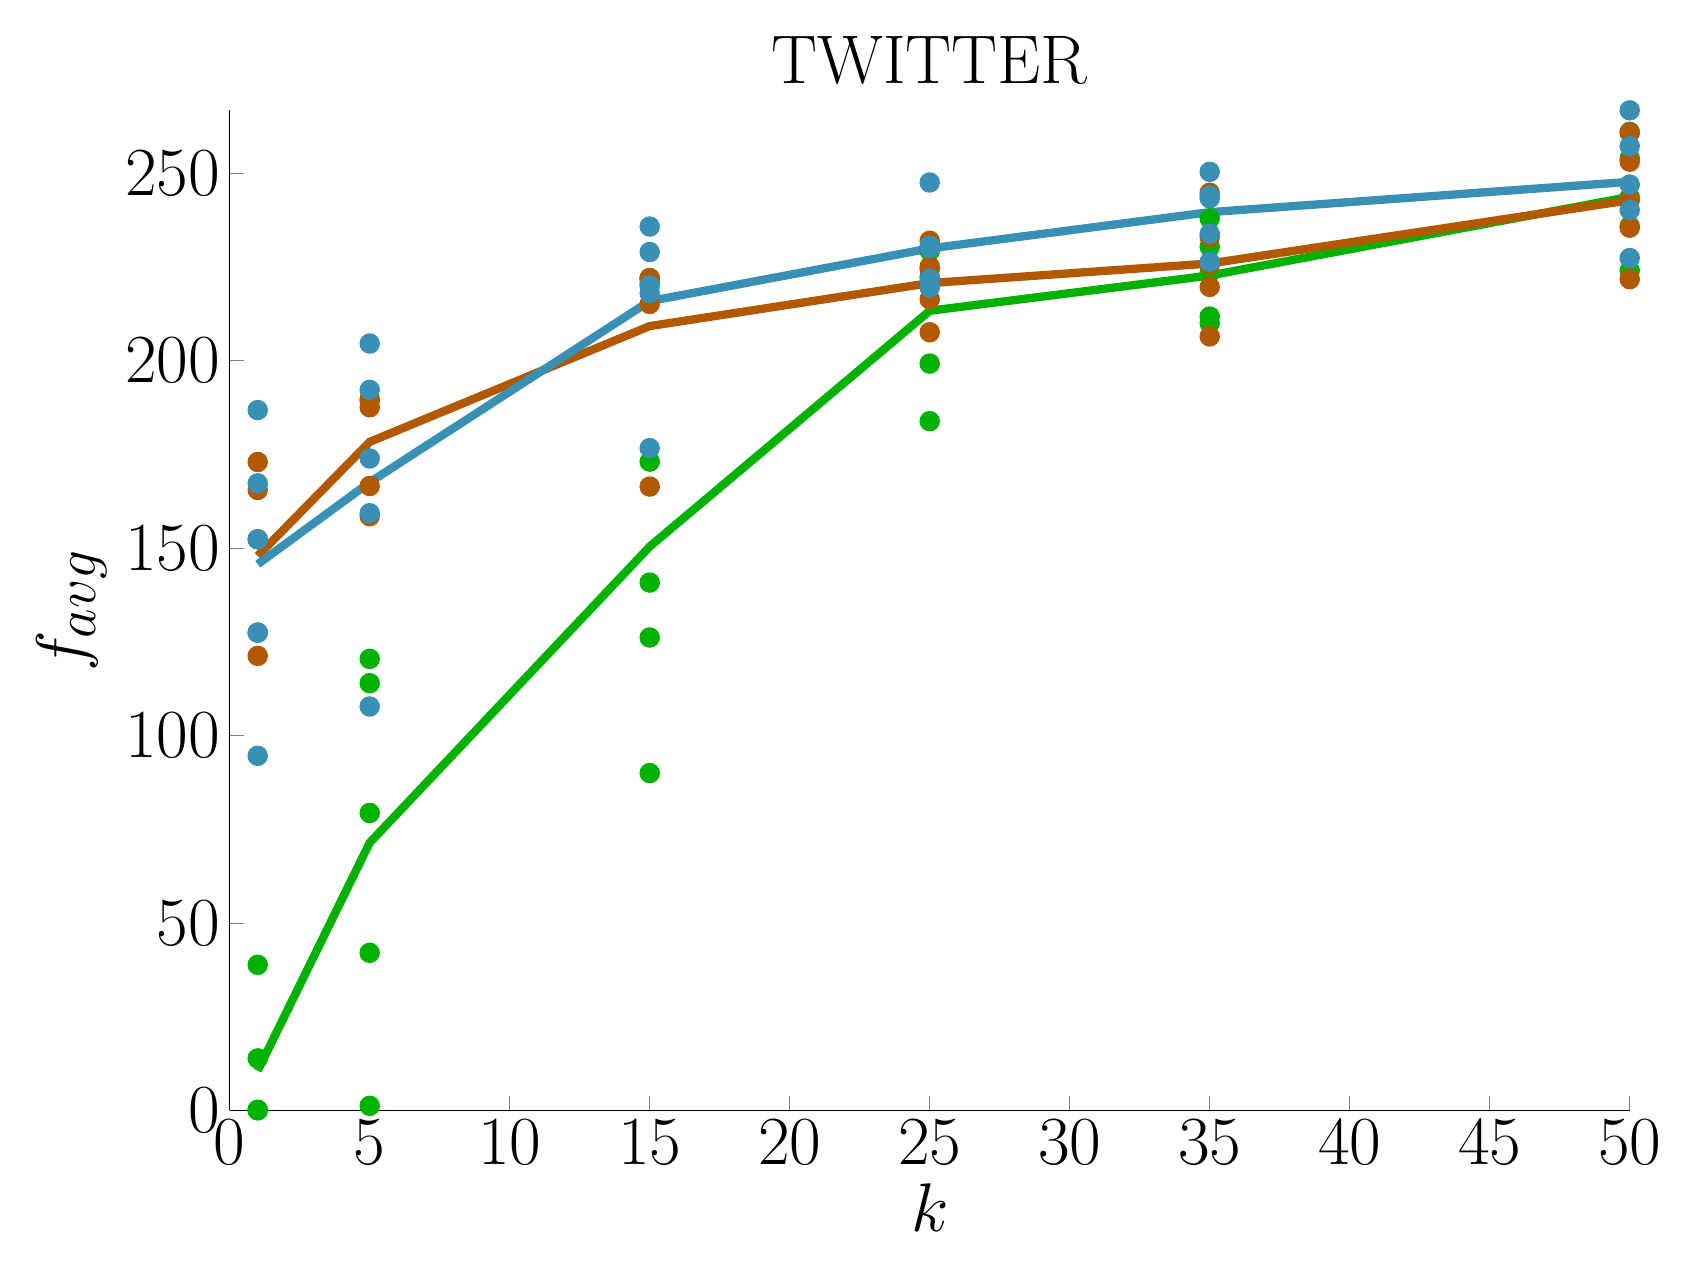
\begin{tikzpicture}

\begin{axis}[%
title style={font=\Huge},
title=TWITTER,
tick label style={font=\Huge},
label style={font=\Huge},
legend style={font=\Huge},
view={0}{90},
max space between ticks=50pt,
width=7in,
height=5in,
scale only axis,
xmin=0, xmax=50,
%xtick={0, 20, 40, 60, 80, 100},
xlabel={$k$},
ymin=0, ymax=266.7,
ylabel={$f_{avg}$},
major tick length=5pt,
axis lines*=left,
legend cell align=left,
clip=false]

\addplot [
only marks,
mark=*,
mark size=3.5pt,
color=green!70!black,
%solid,
%line width=2pt,
]
coordinates{
(1,0.0)(1,0.05)(1,0.15)(1,13.85)(1,38.8)(5,1.2)(5,42.0)(5,79.3)(5,113.9)(5,120.4)(15,89.95)(15,126.1)(15,140.75)(15,173.0)(15,221.95)(25,183.8)(25,199.15)(25,224.35)(25,229.2)(25,229.7)(35,209.95)(35,211.7)(35,223.4)(35,230.3)(35,237.85)(50,223.95)(50,235.8)(50,243.5)(50,253.9)(50,260.95)
};

\addplot [
only marks,
mark=*,
mark size=3.5pt,
color=orange!70!black,
%solid,
%line width=2pt,
]
coordinates{
(1,121.2)(1,127.4)(1,152.3)(1,165.45)(1,172.9)(5,158.45)(5,166.5)(5,187.5)(5,189.2)(5,189.7)(15,166.35)(15,215.05)(15,220.65)(15,221.75)(15,221.95)(25,207.5)(25,216.3)(25,222.35)(25,225.05)(25,231.9)(35,206.4)(35,219.6)(35,225.55)(35,232.95)(35,244.7)(50,221.65)(50,235.4)(50,242.8)(50,253.0)(50,260.75)
};

\addplot [
only marks,
mark=*,
mark size=3.5pt,
color=cyan!70!black,
%solid,
%line width=2pt,
]
coordinates{
(1,94.55)(1,127.4)(1,152.3)(1,167.2)(1,186.75)(5,107.7)(5,159.25)(5,173.85)(5,192.15)(5,204.5)(15,176.6)(15,217.9)(15,220.0)(15,228.9)(15,235.7)(25,219.45)(25,221.8)(25,230.0)(25,230.6)(25,247.45)(35,226.3)(35,233.8)(35,243.25)(35,244.0)(35,250.3)(50,227.3)(50,240.1)(50,246.9)(50,257.15)(50,266.7)
};
p
\addplot [
color=green!70!black,
solid,
line width=3pt
]
coordinates{
(1,10.57)(5,71.36)(15,150.35)(25,213.24)(35,222.64)(50,243.62)
};

\addplot [
color=orange!70!black,
solid,
line width=3pt
]
coordinates{
(1,147.85)(5,178.27)(15,209.15)(25,220.62)(35,225.84)(50,242.72)
};

\addplot [
color=cyan!70!black,
solid,
line width=3pt
]
coordinates{
(1,145.64)(5,167.49)(15,215.82)(25,229.86)(35,239.53)(50,247.63)
};


\end{axis}
\end{tikzpicture}
\end{document}
